\documentclass[usenames,dvipsnames,tikz]{standalone}
\usepackage{xcolor}
\colorlet{tBlue}{RoyalBlue!35!Cerulean}
\colorlet{tRed}{Red}
\usepackage{tikz}
\usepackage{standalone}
\begin{document}
	
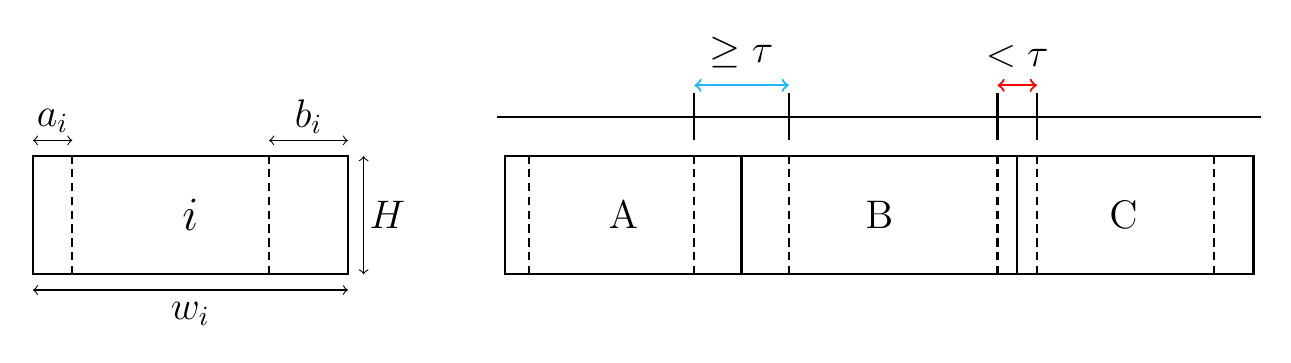
\begin{tikzpicture}
%\draw [help lines] (-1,-2) grid (17,5);

% item i
\draw [thick] (0,0) rectangle (4,1.5);
\draw [thick, densely dashed] (0.5,0) -- (0.5, 1.5);
\draw [thick, densely dashed] (3,0) -- (3, 1.5);
\node at (2,0.75) {\LARGE{$i$}};

%arrow and label for width w_i
\draw [<->] (0,-.2) -- (4,-.2);
\node at (2, -.5) {\Large{$w_i$}};

%arrow and label for score width a_i
\draw [<->] (0, 1.7) -- (0.5, 1.7);
\node at (0.25, 1.95) {\Large{$a_i$}};

%arrow and label for score width b_i
\draw [<->] (3, 1.7) -- (4, 1.7);
\node at (3.5, 2) {\Large{$b_i$}};

%arrow and label for height H
\draw [<->] (4.2,0) -- (4.2,1.5);
\node at (4.5,0.75) {\Large{$H$}};

%-----------------

%3 items ordered
\draw [thick] (6,0) rectangle (15.5,1.5);
%between items A and B
\draw [thick] (9,0) -- (9,1.5);
%between items B and C
\draw [thick] (12.5, 0) -- (12.5,1.5);

%labels for items A, B and C
\node at (7.5,0.75) {\Large{A}};
\node at (10.75,0.75) {\Large{B}};
\node at (13.85,0.75) {\Large{C}};

%score lines for item A
\draw [thick, densely dashed] (6.3,0) -- (6.3,1.5);
\draw [thick, densely dashed] (8.4,0) -- (8.4,1.5);

%score lines for item B
\draw [thick, densely dashed] (9.6,0) -- (9.6,1.5);
\draw [thick, densely dashed] (12.25,0) -- (12.25,1.5);

%score lines for item C
\draw [thick, densely dashed] (12.75,0) -- (12.75,1.5);
\draw [thick, densely dashed] (15,0) -- (15,1.5);

%------------------

%Bar with knives 
\draw [thick] (5.9,2) -- (15.6,2);

%knives for items A and B
\draw [thick] (8.4,1.7) -- (8.4,2.3);
\draw [thick] (9.6,1.7) -- (9.6,2.3);

%knives for items B and C
\draw [thick] (12.25,1.7) -- (12.25,2.3);
\draw [thick] (12.75,1.7) -- (12.75,2.3);


%constraint label for score widths between items A and B (feasible, >= tau)
\draw [thick, <->, tBlue] (8.4, 2.4) -- (9.6, 2.4);
\node [above] at (9,2.5) {\Large{$\geq \tau$}};

%constraint label for score widths between items B and C (infeasible, < tau)
\draw [thick, <->, tRed] (12.25, 2.4) -- (12.75, 2.4);
\node [above] at (12.5,2.5) {\Large{$< \tau$}};

%\draw [<->] (3.5,2.2) -- (4.5,2.2);
%\node at (4, -.4) {\scriptsize $\geq \tau$};

\end{tikzpicture}
	
\end{document}